%!TeX root = SAS2017_18_senacheribbe.tex

\newcommand{\wc}{\omega_c}
\newcommand{\dt}{\Delta_t}
\newcommand{\zi}{z^{-1}}
\newcommand{\zii}{z^{-2}}

\graphicspath{{graphics/task2/}}
\chapter{Task 2: implementation of discrete-time low-pass Butterworth filter}
\section{Description of the task}
The aim of this task is to implement a third order low-pass Butterworth filter in discrete time using the bilateral transformation. The analog transfer function is given by
\begin{equation}\label{eq:t2_analog_tf_text}
H_a(s)=\frac{\wc^3}{(s-p_1)(s-p_2)(s-p_3)}, \quad p_1=-\wc, p_2=-\wc e^{j\pi/3}, p_2=-\wc e^{-j\pi/3}
\end{equation}
The derivation of the digital transfer function must be performed analytically and then the filter has to be coded into MATLAB for an angular frequency $\wc=20$ ($\wc$ must be left as parameter).\\
The impulse response must be evaluated analytically for the analog filter and compared with the one of the discrete-time filter.
The frequency behavior of the digital implementation should then be compared using the DTFT and FFT against the frequency response of the analog equivalent.
Finally the energy of the impulse response of the filter must be computed both analytically from the analog tf and using the discrete-time impulse response of the filter (in time and frequency domain).
\section{MATLAB code}
\lstinputlisting[style= Matlab-editor,  basicstyle=\small]{../final_project_task2.m}

\pagebreak
\section{Results and comments}
\subsection{Derivation of the discrete-time transfer function}
We can rewrite \cref{eq:t2_analog_tf_text} by multiplying the two complex conjugate poles and getting a real-coefficients second order term
\begin{equation}\label{eq:t2_analog_tf}
%%H_a(s)=\frac{\wc^3}{(s+\wc)(s^2+\wc^2+s\wc)}= \underbrace{\dfrac{\wc}{(s+\wc)}}_{H_1(s)} \underbrace{\dfrac{\wc^2}{(s^2+\wc^2+s\wc)}}_{H_2(s)}
H_a(s)=\frac{\wc^3}{(s+\wc)(s^2+\wc^2+s\wc)}=\dfrac{\wc}{(s+\wc)}\,\dfrac{\wc^2}{(s^2+\wc^2+s\wc)}=H_{a1}(s)\, H_{a2}(s)
\end{equation}
\\
From \cref{eq:t2_analog_tf}, the substitution for the bilinear transformation is applied considering separately $H_{a1}(s)$ and $H_{a2}$.
\begin{align}
H_{a1}(s)=&\dfrac{\wc}{(s+\wc)}, \quad s\leftarrow \frac{2}{\dt}\frac{1-\zi}{1+\zi} \quad \implies \nn \\
H_1(z)=&\frac{Y(z)}{X(z)}=\frac{\wc\dt (1+\zi)}{\zi(-2+\wc\dt)+2+\wc\dt} \label{eq:t2_h1} \\
&Y(z)=\underbrace{\frac{\wc\dt}{2+\wc\dt}}_{A}  (X(z)+\zi X(z))+\underbrace{\frac{2-\wc \dt}{2+\wc \dt}}_{B} \zi Y(z) \label{eq:t2_d_1o} \\
\nn\\
H_{a2}(s)=&\dfrac{\wc^2}{(s^2+\wc^2+s\wc)}, \quad s\leftarrow \frac{2}{\dt}\frac{1-\zi}{1+\zi} \quad \implies \nn \\
H_2(z)=&\frac{Y(z)}{X(z)}= \frac{\wc^2\dt^2(1+2\zi+\zii)}{\zii (4+\wc^2 \dt^2-2\wc\dt)+ \zi (-8+2\wc^2\dt^2)+4+\wc^2\dt^2+2\wc\dt} \label{eq:t2_h2}  \\
&\begin{aligned}
Y(z)&=\underbrace{\frac{\wc^2 \dt^2}{4+\wc^2 \dt^2+2\wc\dt}}_{C}(1+ 2 \zi +\zii) X(z) +\underbrace{\frac{8-2\wc^2\dt^2}{4+\wc^2\dt^2+2\wc\dt}}_{D} \zi Y(z)\\
&+\underbrace{\frac{-4-\wc^2\dt^2+2\wc\dt}{4+\wc^2\dt^2+2\wc\dt}}_{E} \zii Y(z) \label{eq:t2_d_2o}
\end{aligned}
\end{align}
\\
The finite difference equations corresponding to \cref{eq:t2_d_1o,eq:t2_d_2o} are coded into MATLAB in cascade. The angular frequency $\wc$ is kept as parameter that can be varied to change the cutoff frequency of the filter. The block diagram of the digital filter is presented in \cref{fig:t2_block_diagram}.
\\
\begin{figure} [H]
	\centering
	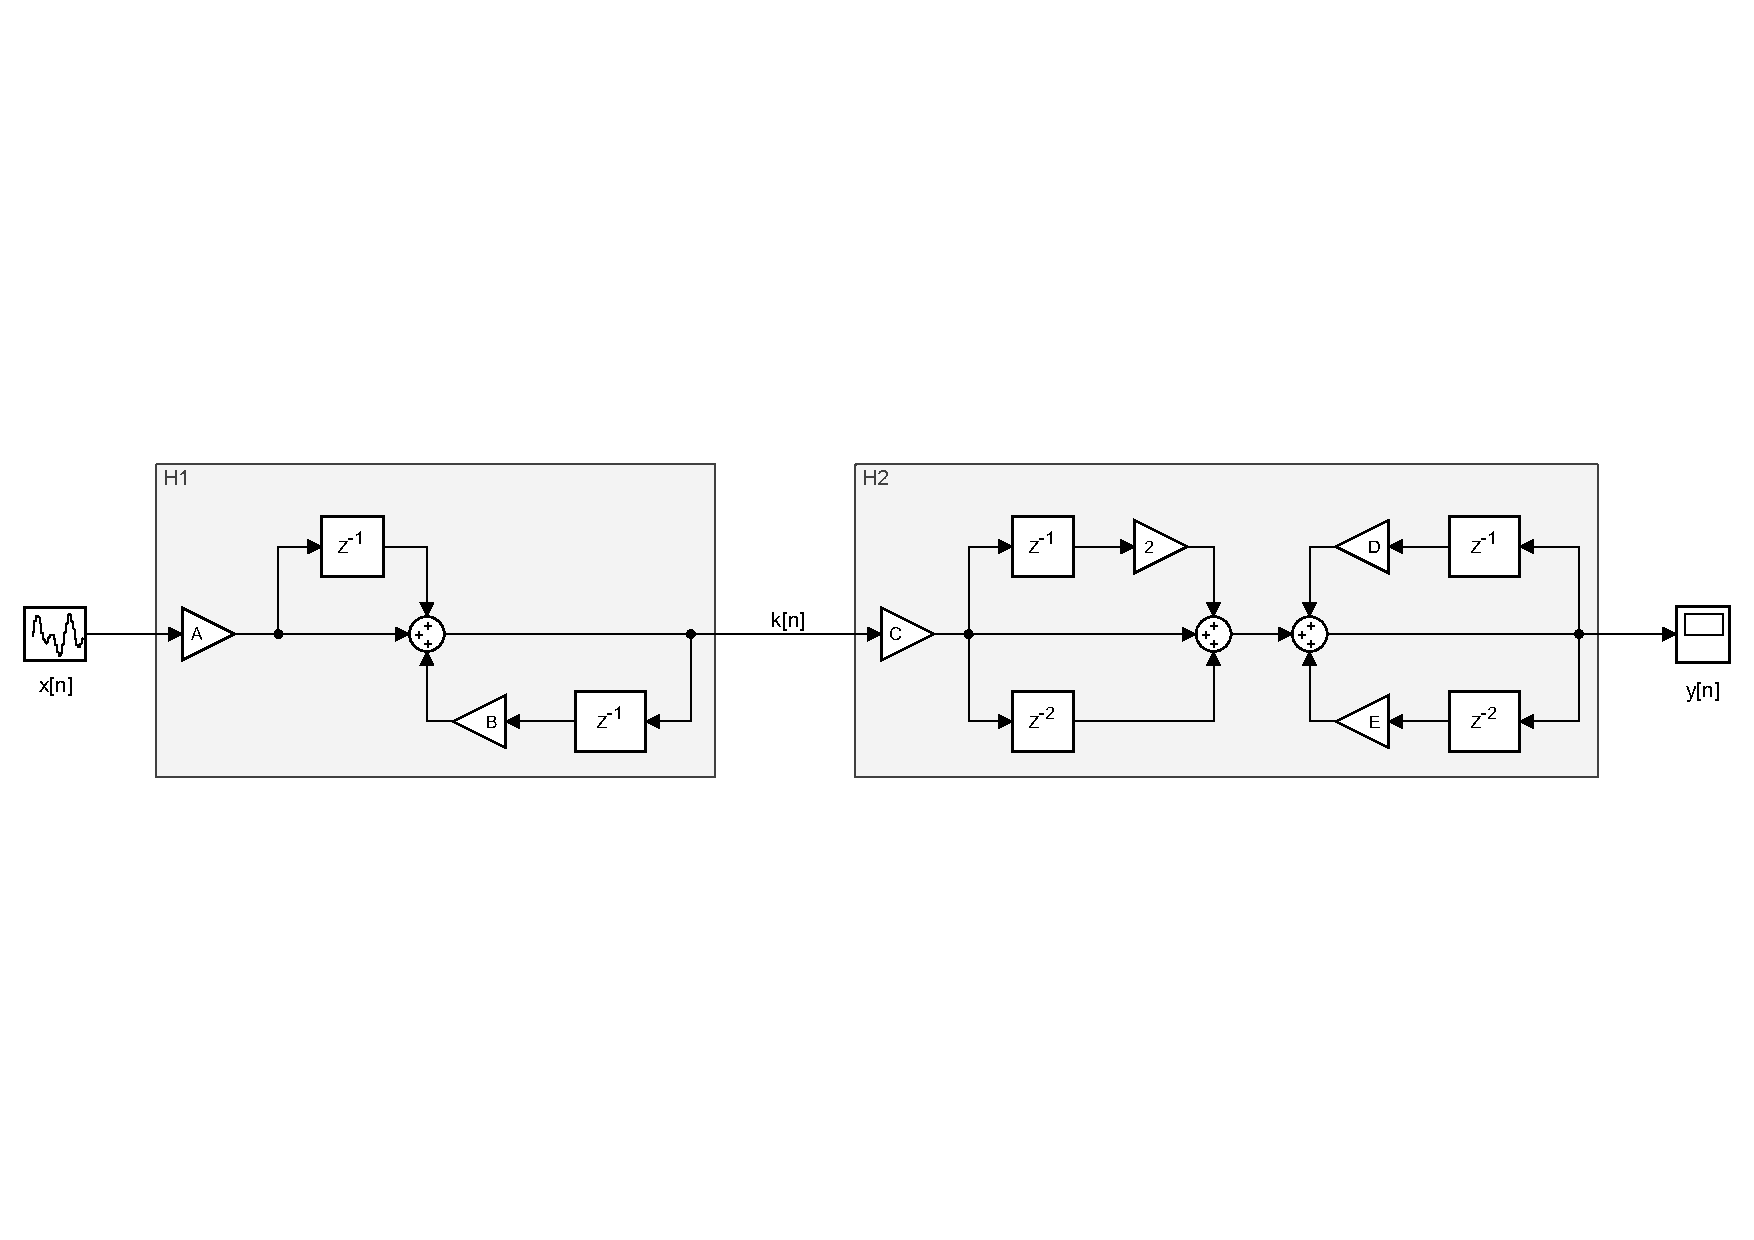
\includegraphics[trim={0cm 7.5cm 0cm 7.5cm}, clip, width=\linewidth]{block_diagram}
	\caption{Block diagram of the filter - the constants \textit{A, B, C, D, E} are reported in \cref{eq:t2_d_1o} and \cref{eq:t2_d_2o}}
	\label{fig:t2_block_diagram}
\end{figure}


\subsection{Impulse response}
In order to evaluate the impulse response of the analog filter, we compute the residues of \cref{eq:t2_analog_tf}, getting the following result
\begin{gather}
H_a(s)=\frac{\wc}{s+\wc}+\frac{\wc \frac{\sqrt 3}{3} e^{j \frac{5 }{6}\pi}}{s+\wc e^{j \frac{\pi}{3}}} + cc \implies \nn \\
h_a(t)=\left(\wc e^{-\wc t} + 2 \wc \frac{\sqrt 3}{3} e^{-\wc \frac{1}{2} t}  cos\left(-\frac{\sqrt 3}{2} \wc t + \frac{5}{6} \pi\right)\right) u (t) \label{eq:t2_analog_impulse}
\end{gather}
\\
The impulse response of the digital filter is instead obtained by evaluating the output of the filter with a discrete delta function as input.
Both the continuous (\cref{eq:t2_analog_impulse}) and discrete responses are shown in \cref{fig:t2_impulse_resp}. By setting the filter parameter $\dt=\SI{0.005}{s}$, the two plots are coincident.
%https://www.wolframalpha.com/input/?i=integrate+a+e%5E(-ax)%2B2+a+sqrt(3)%2F3+*e%5E(-a%2F2+x)(cos(-sqrt(3)*a%2F2*x%2B5%2F6pi))+from+0+to+inf

\begin{figure} [H]
	\centering
	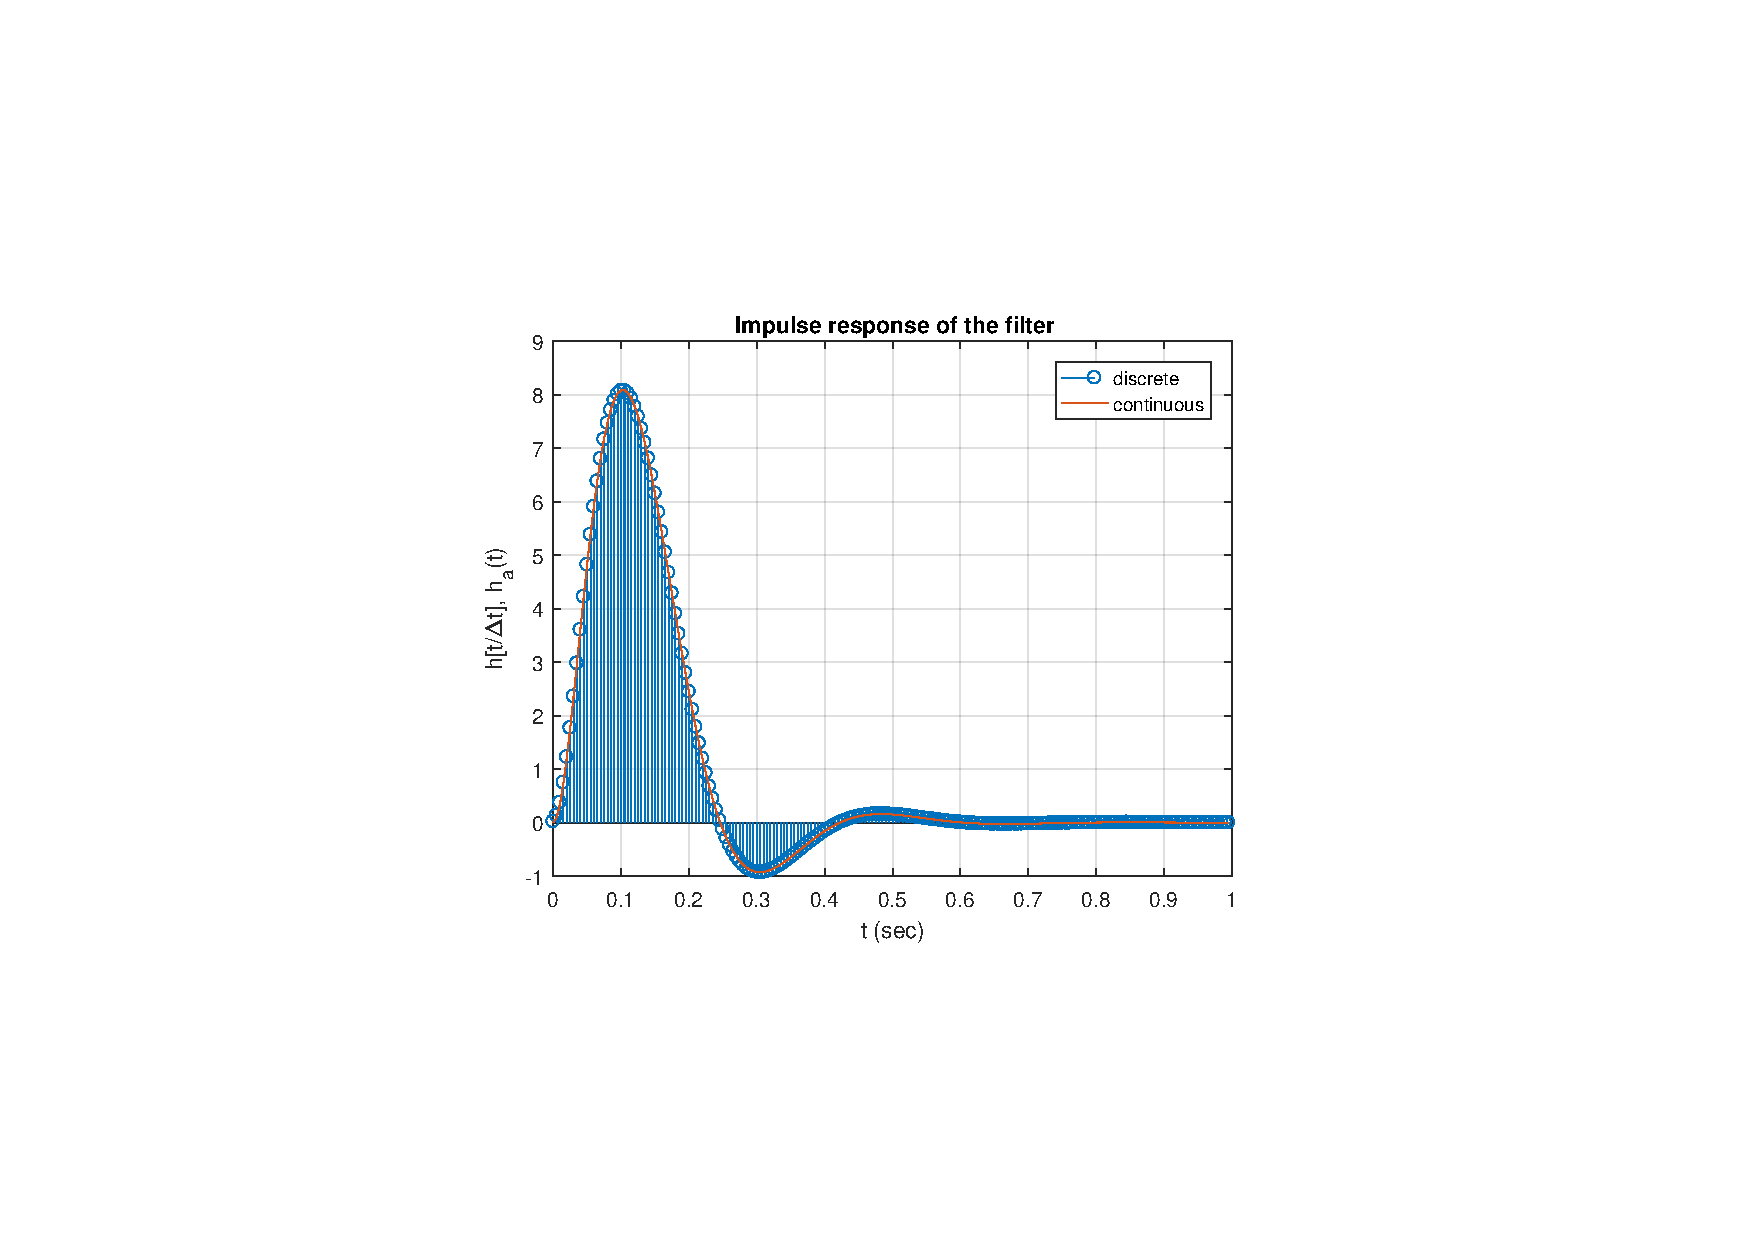
\includegraphics[trim={8cm 4.8cm 8cm 5cm}, clip, width=0.8\linewidth]{impulse_resp}
%%	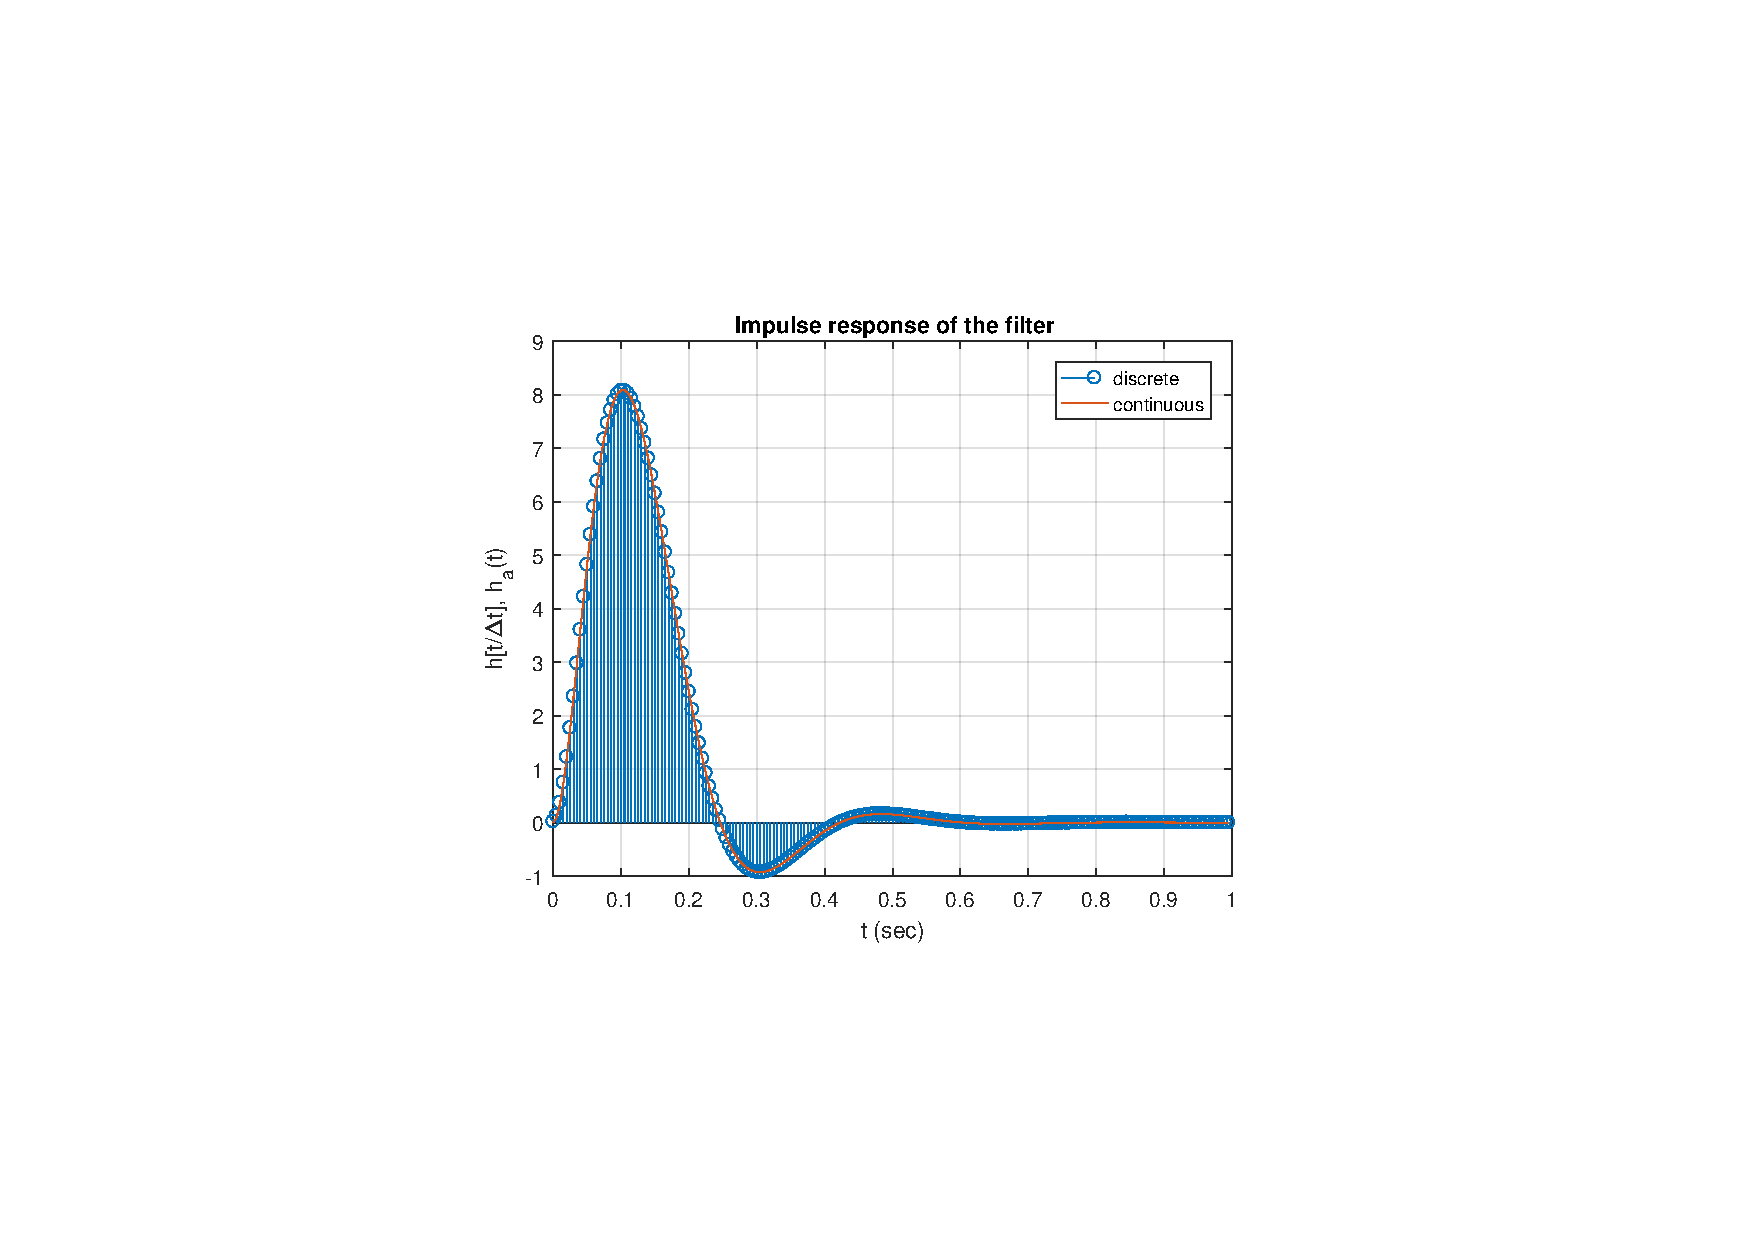
\includegraphics[trim={3cm 1.5cm 3cm 1cm}, clip, width=\linewidth]{impulse_resp}
	\caption{Impulse response of the filter - the analog and digital responses are coincident}
	\label{fig:t2_impulse_resp}
\end{figure}
\pagebreak
\subsection{Frequency response}
The frequency response of the analog filter is given by
\begin{equation}\label{eq:t2_afourier}
|H_a(f)|^2=\frac{\wc^6}{\wc^6+(2 \pi f)^2} 
\end{equation}
To prove this result we start from \cref{eq:t2_analog_tf} and using $H_a^*(j2\pi f)=H_a(-j2\pi f)$ we get
\begin{align*}
|H_a(f)|^2&=H_a(j2\pi f) H_a^*(j2\pi f)=H_a(j2\pi f) H_a(-j2\pi f)\\
&=\frac{\wc^6}{(\wc+2j\pi f)(\wc-2j\pi f)(-4\pi^2f^2+\wc^2-j2\pi f\wc)(-4\pi^2f^2+\wc^2+j2\pi f\wc)}\\
&=\frac{\wc^6}{(\wc^2+4\pi^2 f^2)(\wc^4+16\pi^4f^4-4\pi^2 f^2 \wc^2)}\\
&=\frac{\wc^6}{(\wc^2)^3+(4 \pi^2 f^2)^3}
\end{align*}
\\
For the digital filter, the DTFT is computed numerically using MATLAB, starting from the transfer function of the filter in the z-domain (\cref{eq:t2_h1,eq:t2_h2}) as following
\begin{equation*}
DTFT[f]=H (e^{j 2 \pi f \dt} )=H_1 (e^{j 2 \pi f \dt} ) H_2 (e^{j 2 \pi f \dt })
\end{equation*}
\\
The modulus of DTFT is plotted in \cref{fig:t2_dtft_lin,fig:t2_dtft_log} and compared with $|H_a(f)|$ (from \cref{eq:t2_afourier}). The graphs are coincident around frequency 0, but they differ at around $1/(2\dt)=\SI{100}{\hertz}$ (clearly visible on the semilog plot). This is due to frequency warping, since the continuous frequency range $[-\infty, +\infty]$ is compressed on the range $\left [-\frac{1}{2\dt}, \frac{1}{2\dt}\right ]$ for the discrete filter. To reduce this effect, a smaller value for $\dt$ can be chosen or some pre-warping techniques may be applied.
%https://en.wikipedia.org/wiki/Bilinear_transform#Frequency_warping
\begin{figure} [H]
	\centering
	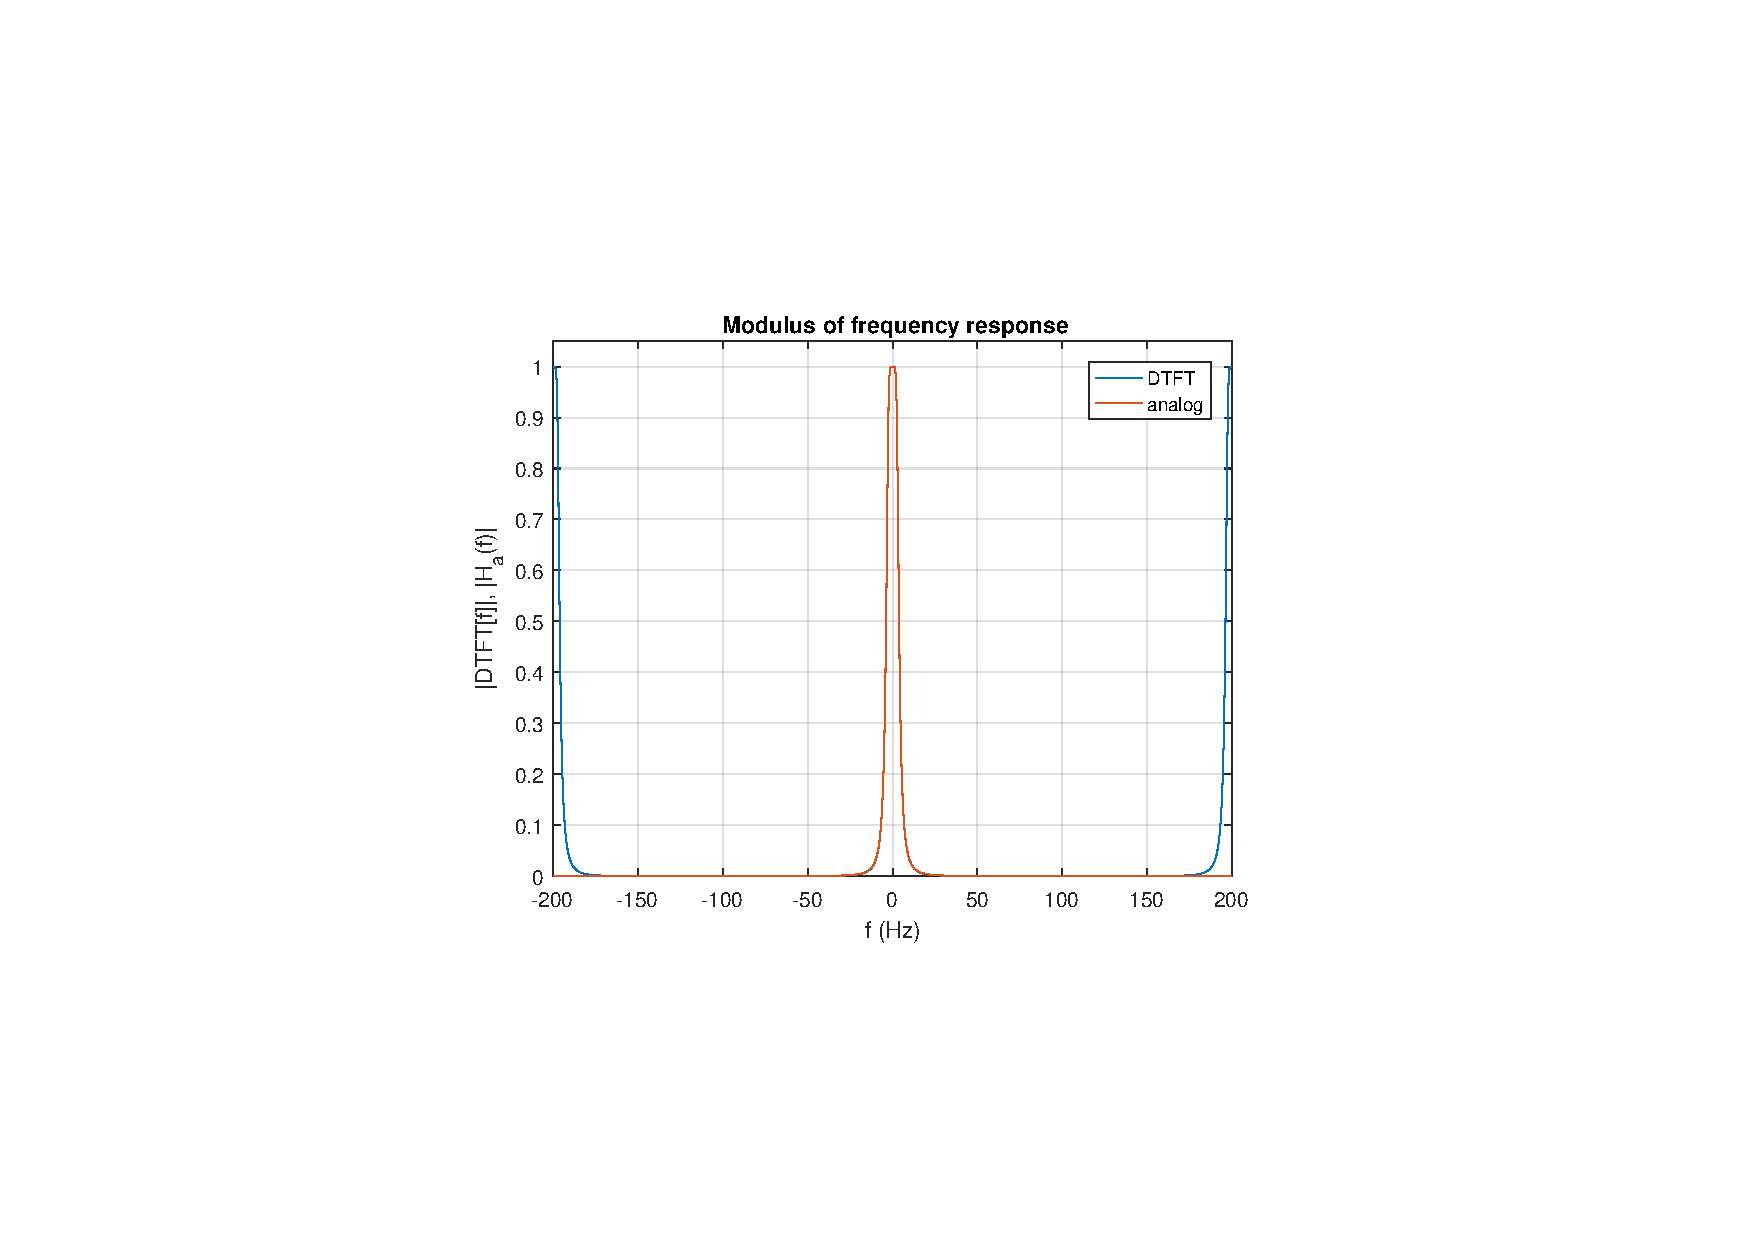
\includegraphics[trim={8cm 4.8cm 8cm 5cm}, clip, width=0.8\linewidth]{frequency_resp_lin}
	%%	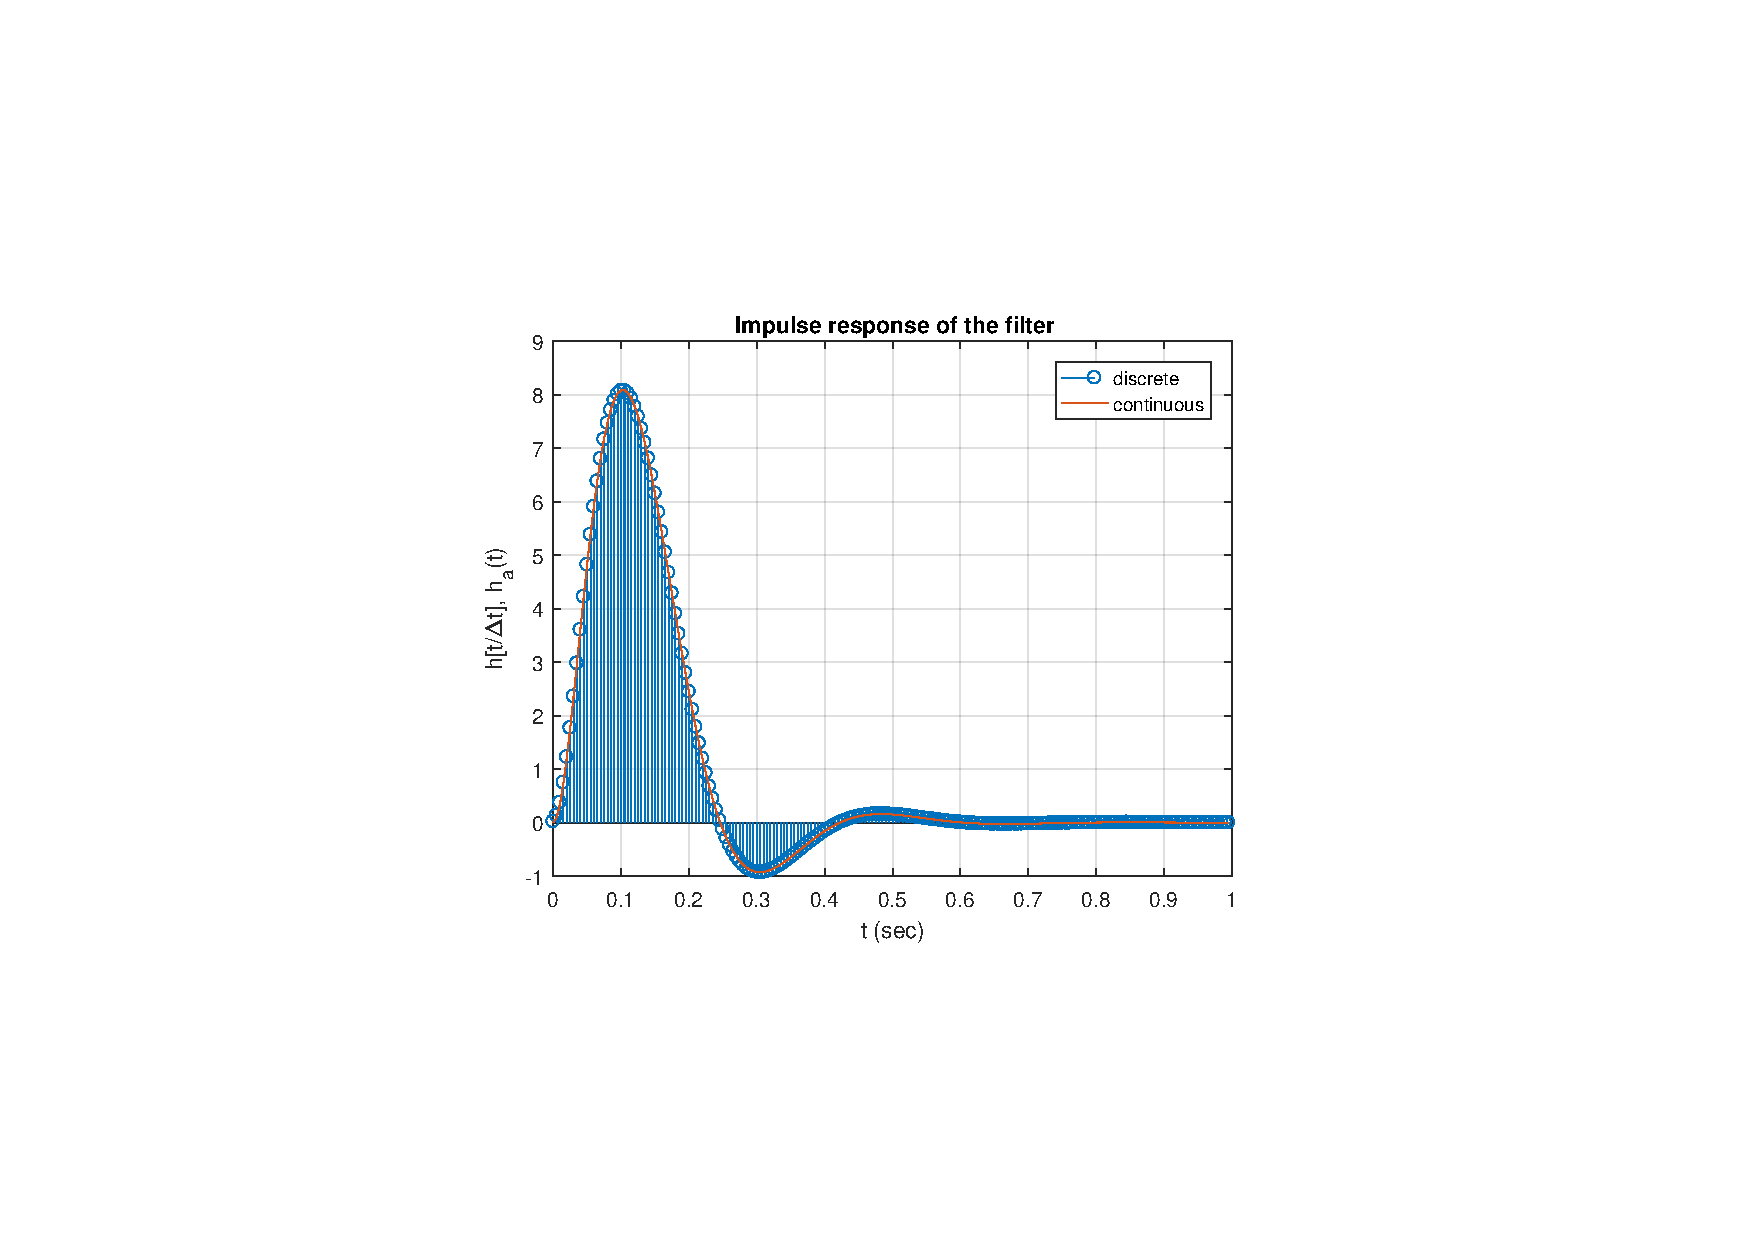
\includegraphics[trim={3cm 1.5cm 3cm 1cm}, clip, width=\linewidth]{impulse_resp}
	\caption{Modulus of frequency response - the periodicity of the DTFT is clearly visible}
	\label{fig:t2_dtft_lin}
\end{figure}
\begin{figure} [H]
	\centering
	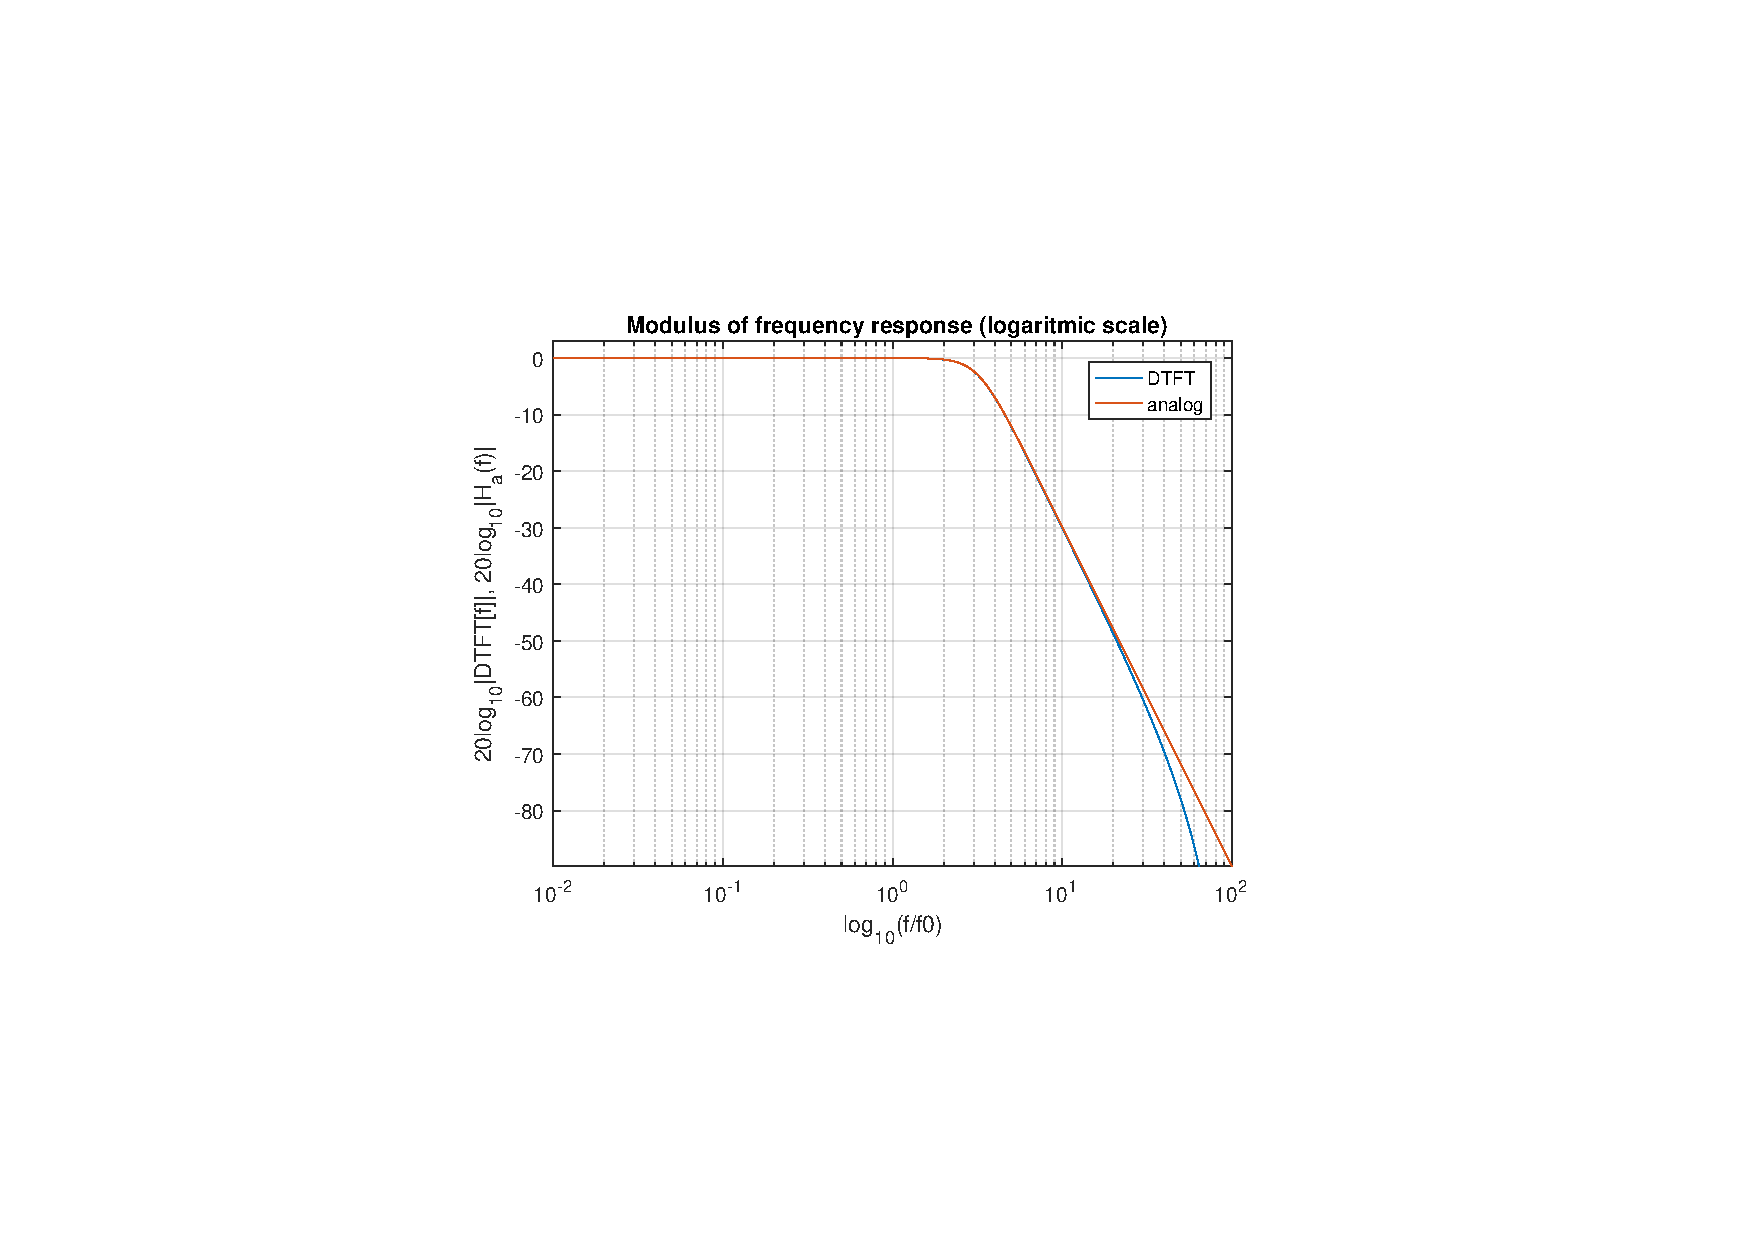
\includegraphics[trim={8cm 4.8cm 8cm 5cm}, clip, width=0.8\linewidth]{frequency_resp_log}
	%%	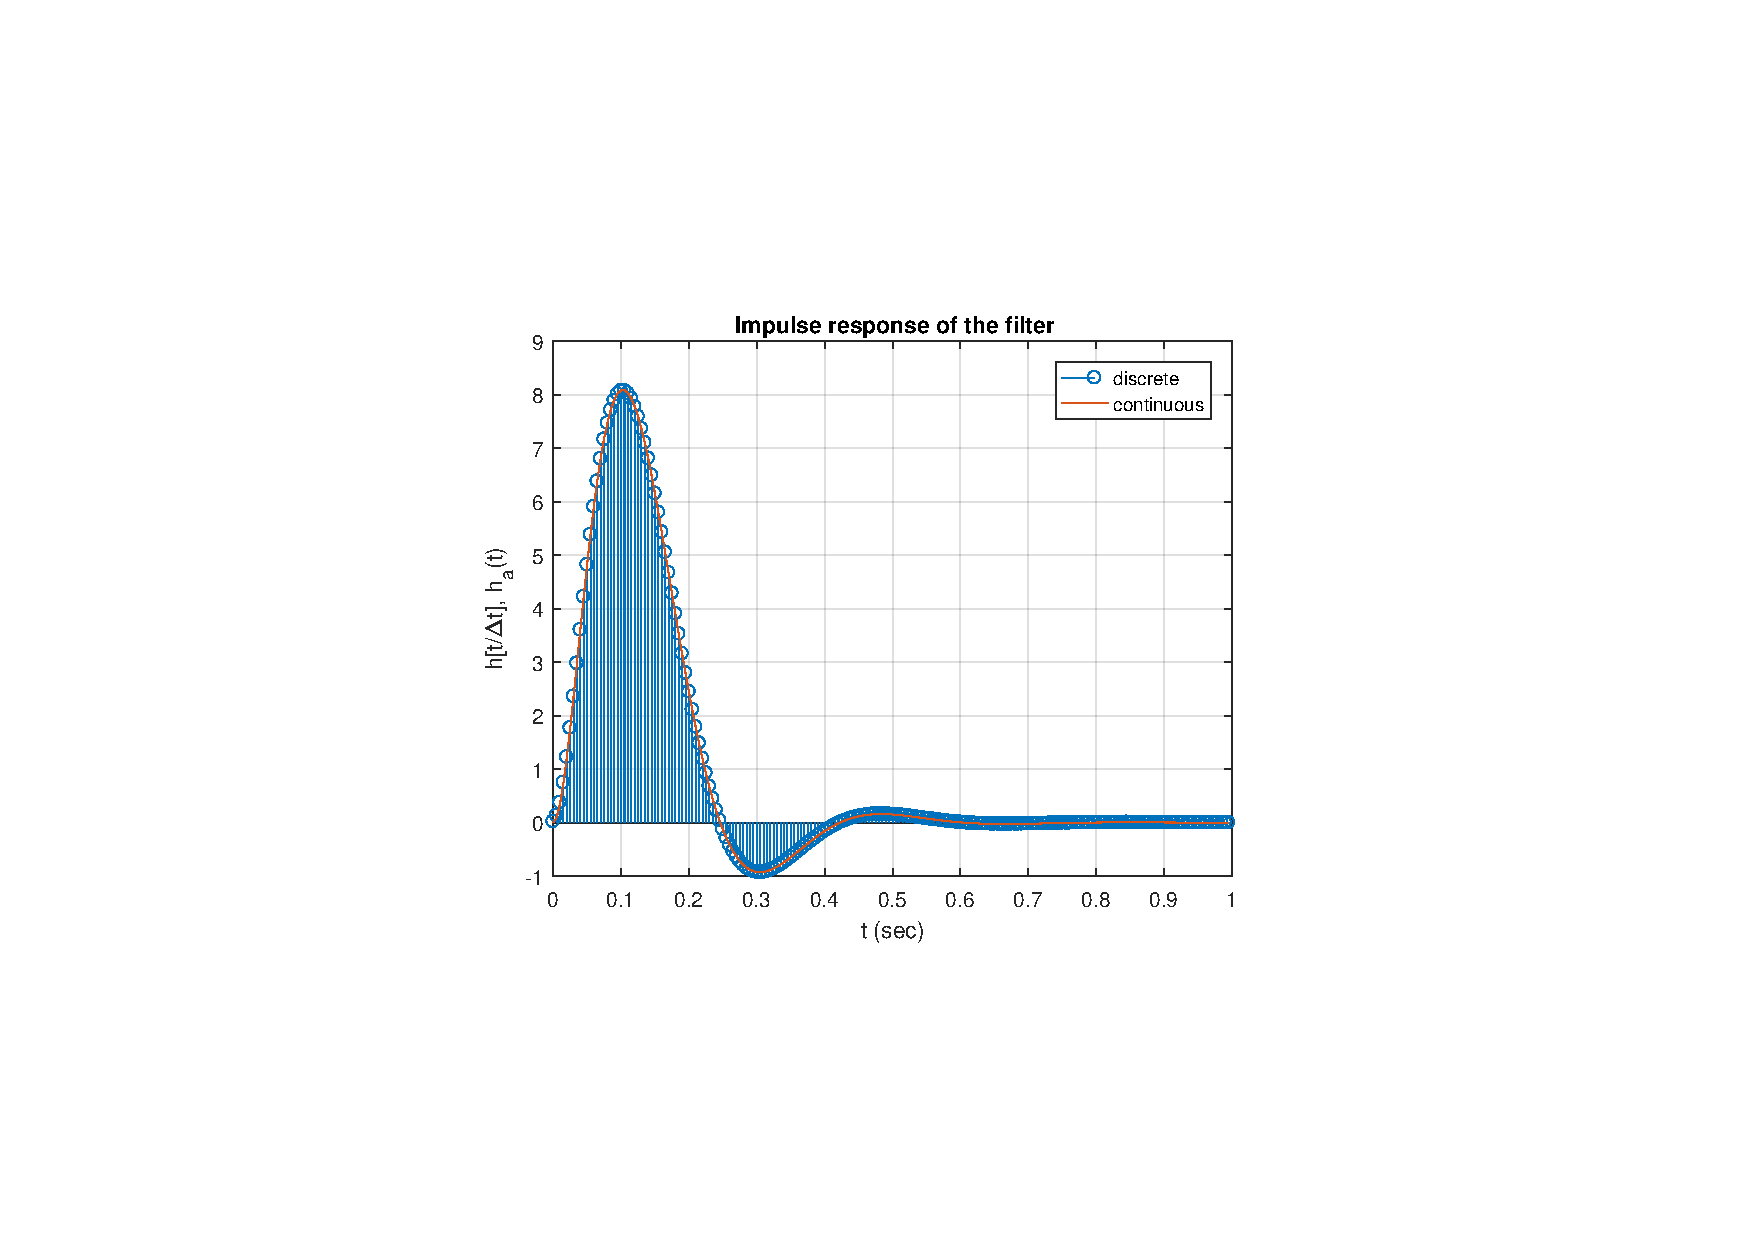
\includegraphics[trim={3cm 1.5cm 3cm 1cm}, clip, width=\linewidth]{impulse_resp}
	\caption{Modulus of frequency response (semi log) - the frequency warping effect can be noticed at $\approx \SI{100}{\hertz}$}
	\label{fig:t2_dtft_log}
\end{figure}
The frequency behavior of the digital filter can also be evaluated from the FFT of the impulse response of the discrete filter, computing it using MATLAB function \textit{fft()} and then shifting it around frequency zero. The plots in \cref{fig:t2_fft,fig:t2_fft_log} show again the frequency warping effect around $1/(2\dt)$.
\begin{figure}
	\centering
	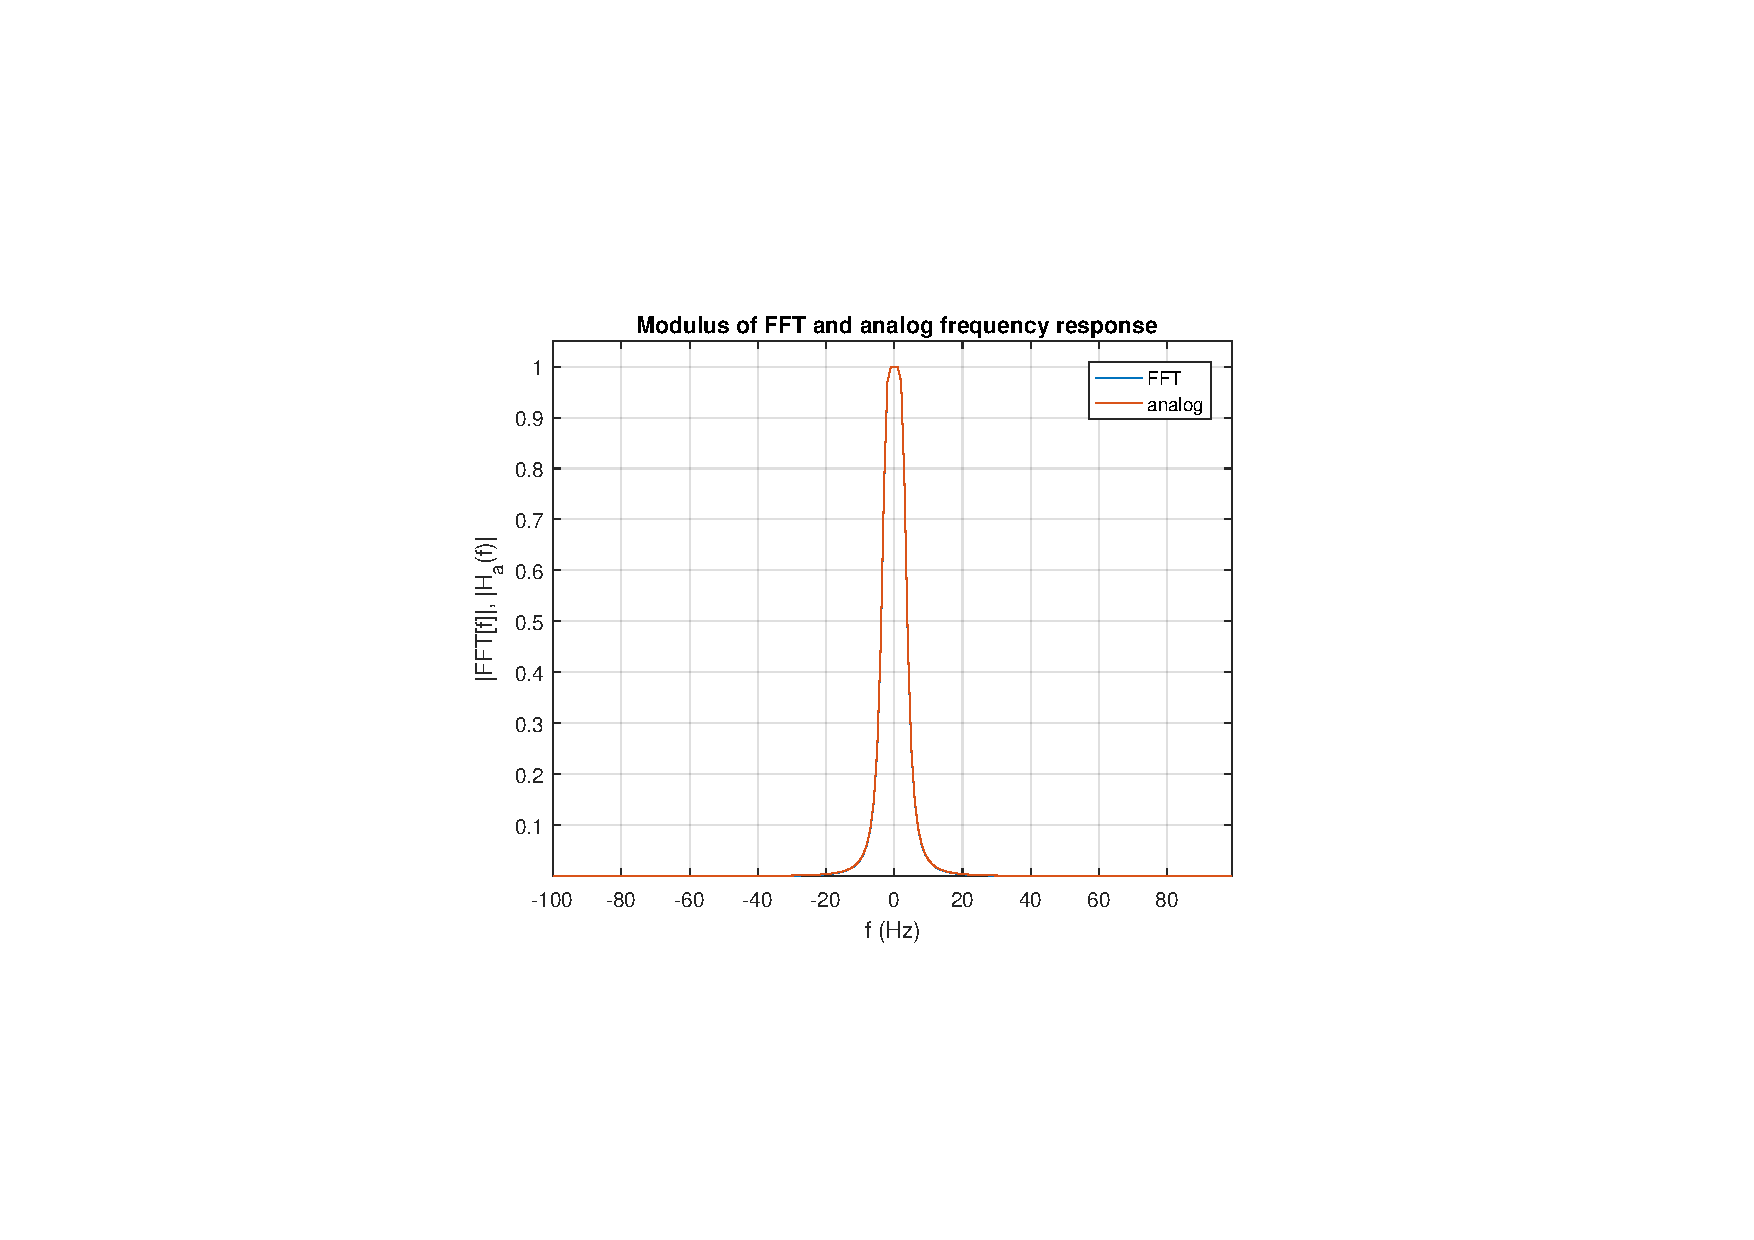
\includegraphics[trim={8cm 4.8cm 8cm 5cm}, clip, width=0.8\linewidth]{fft}
	%%	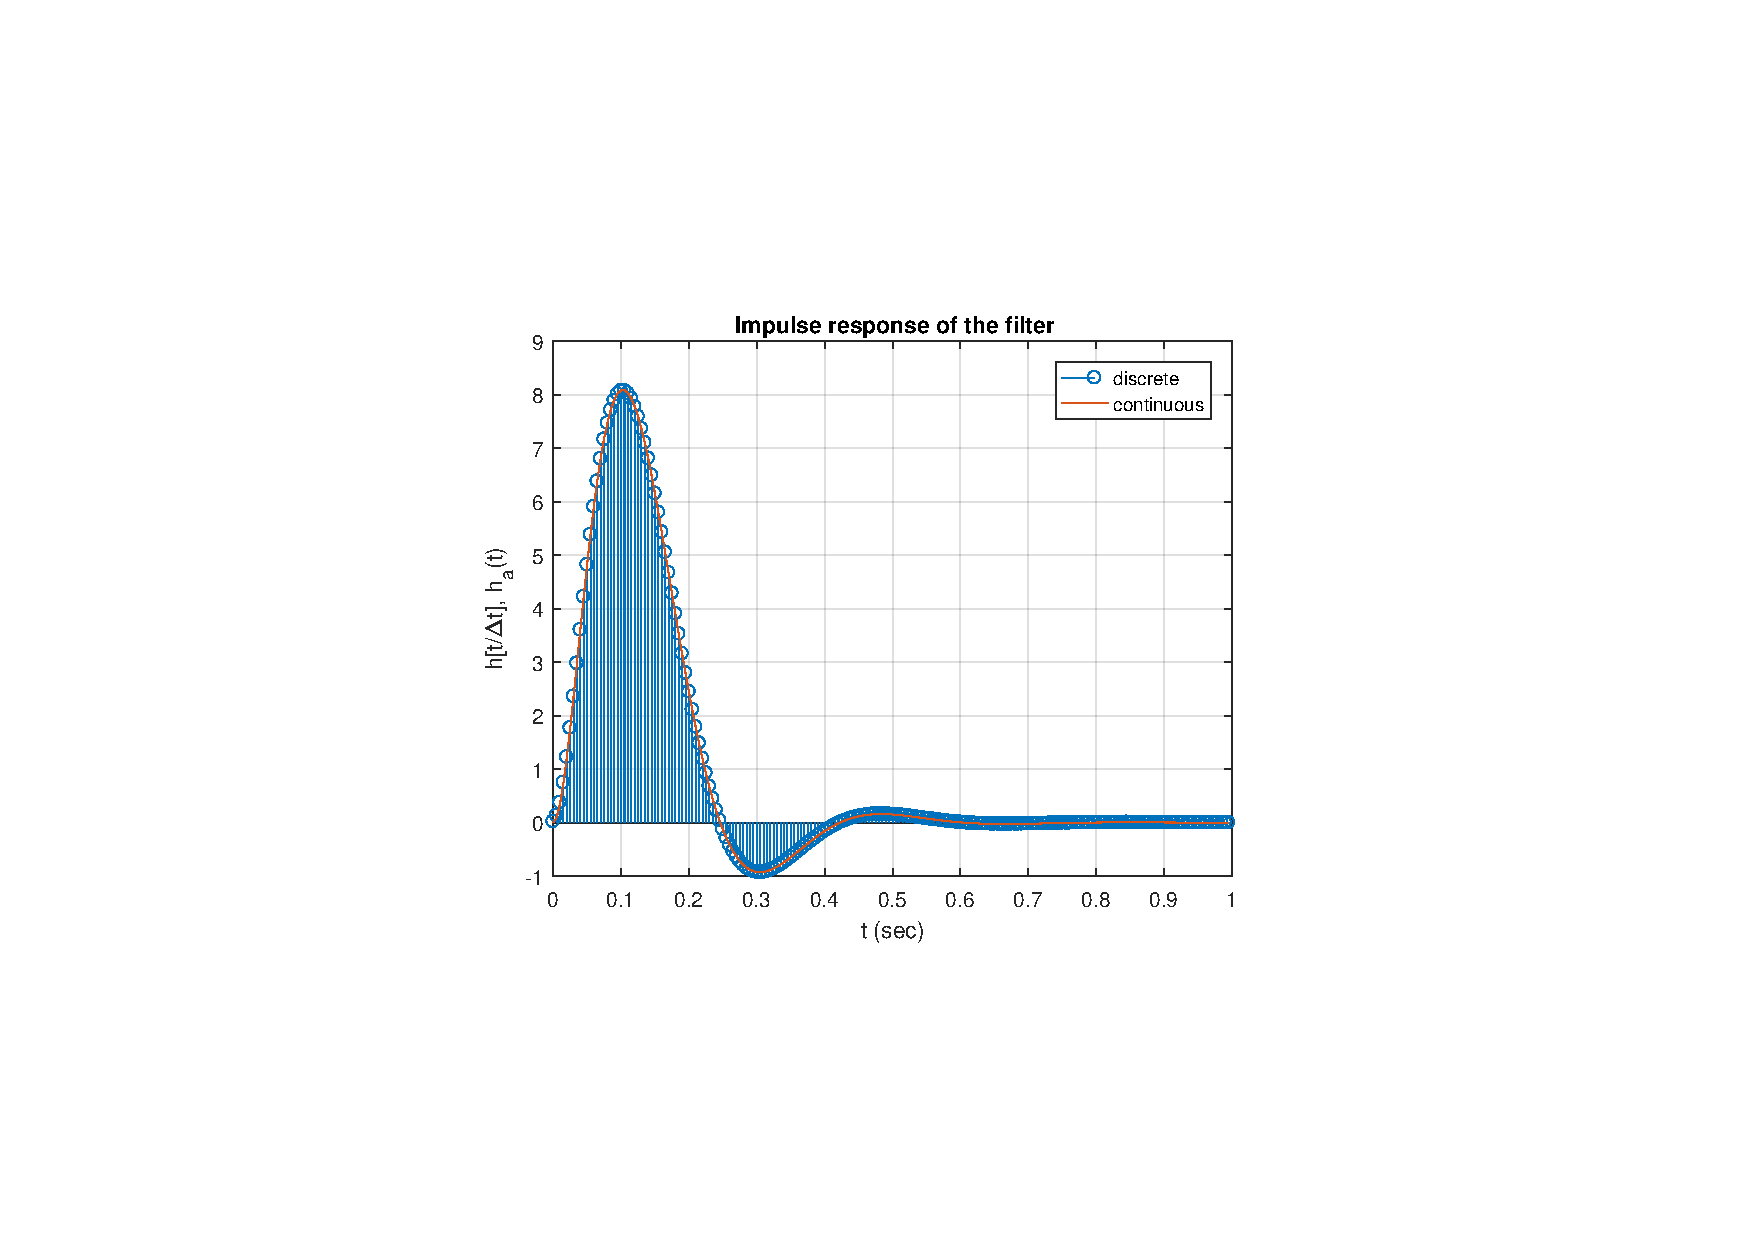
\includegraphics[trim={3cm 1.5cm 3cm 1cm}, clip, width=\linewidth]{impulse_resp}
	\caption{FFT of the impulse response (linear scale)}
	\label{fig:t2_fft}
\end{figure}
\begin{figure}
	\centering
	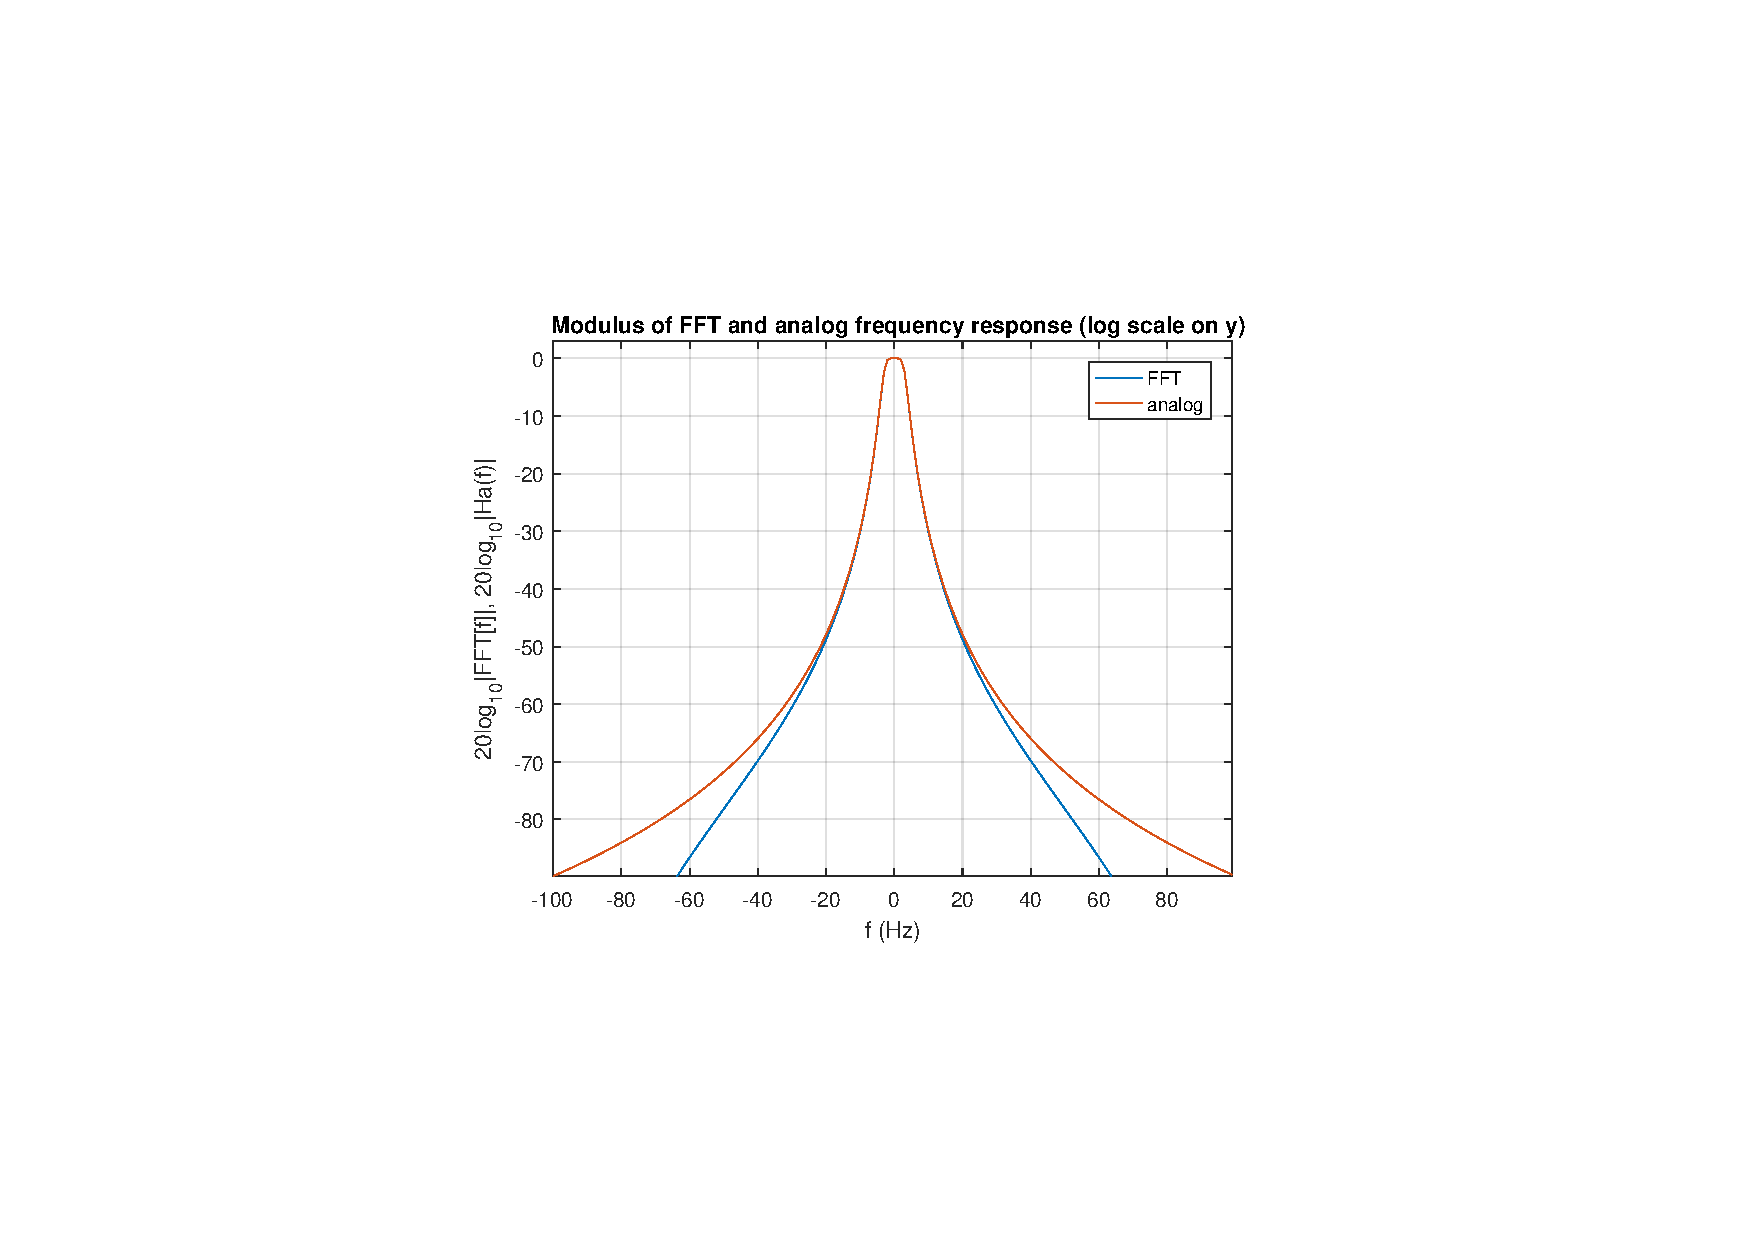
\includegraphics[trim={8cm 4.8cm 8cm 5cm}, clip, width=0.8\linewidth]{fft_log}
	%%	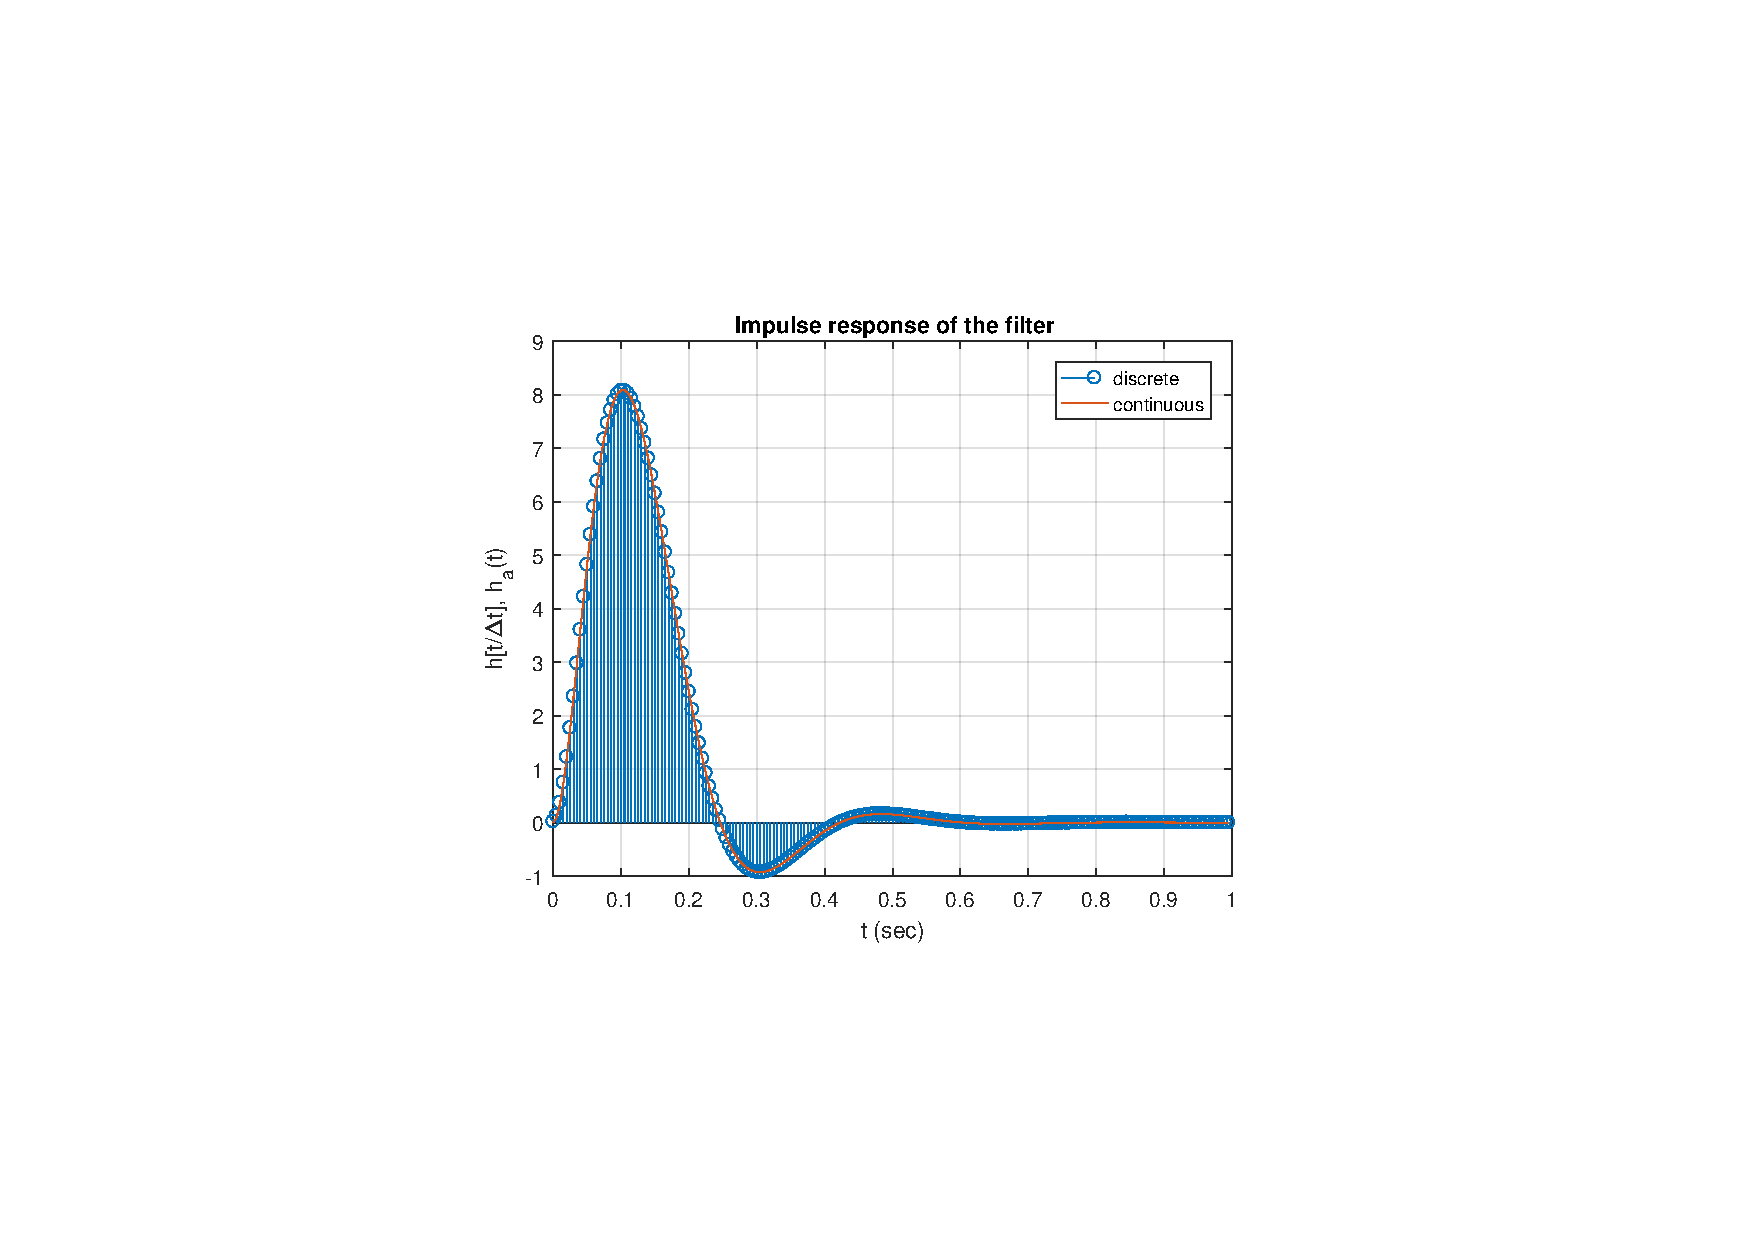
\includegraphics[trim={3cm 1.5cm 3cm 1cm}, clip, width=\linewidth]{impulse_resp}
	\caption{FFT of the impulse response (log scale on y) - the warping effect is again visible around \SI{100}{\hertz}}
	\label{fig:t2_fft_log}
\end{figure}

\subsection{Energy of impulse response}
The energy of the analog impulse response $h_a(t)$ was computed analytically using Wolfram$|$Alpha and the result confirmed using numerical integration in MATLAB: 
\begin{equation} \label{eq:t2_a_energy}
\mathcal{E}(h_a(t))=\int_{0}^{+\infty} |h_a(t)|^2 =\frac{20}{3}\approx 6.6667
\end{equation}
%https://www.wolframalpha.com/input/?i=integrate+(20+e%5E(-20x)%2B2+20+sqrt(3)%2F3+*e%5E(-20%2F2+x)(cos(-sqrt(3)*20%2F2*x%2B5%2F6pi)))%5E2+from+0+to+inf
%https://www.wolframalpha.com/input/?i=integrate+(a+e%5E(-ax)%2B2+a+sqrt(3)%2F3+*e%5E(-a%2F2+x)(cos(-sqrt(3)*a%2F2*x%2B5%2F6pi)))%5E2+from+0+to+inf
On the other hand, the energy computed from the time discrete impulse response and from its FFT is 
\begin{equation}
\mathcal{E}(h[n])=\mathcal{E}(FFT[k])=6.6584
\end{equation}
which is compatible with the result of the analog response in \cref{eq:t2_a_energy}.
